\documentclass{easychair}

% \usepackage{doc}
\usepackage{setspace}
\usepackage{verbatim}
\usepackage{wasysym}

%----Making things more compact
\newcommand{\smalltt}[1]{\small \texttt{#1}}
\newenvironment{packed_itemize}{
\vspace*{-0.2em}
\begin{itemize}
\setlength{\partopsep}{0pt}
\setlength{\itemsep}{1pt}
\setlength{\parskip}{0pt}
\setlength{\parsep}{0pt}
}{\end{itemize}}
\newenvironment{packed_enumerate}{
\vspace*{-0.2em}
\begin{enumerate}
\setlength{\partopsep}{0pt}
\setlength{\itemsep}{1pt}
\setlength{\parskip}{0pt}
\setlength{\parsep}{0pt}
}{\end{enumerate}}
% \renewcommand{\textfraction}{0.07}
% \renewcommand{\topfraction}{0.9}
% \renewcommand{\bottomfraction}{0.9}
% \renewcommand{\floatpagefraction}{0.66}
% \setlength{\floatsep}{2.0pt plus 2.0pt minus 2.0pt}
% \setlength{\textfloatsep}{5.0pt plus 2.0pt minus 0.0pt}

\title{Stepping Stones in the TPTP World}

\author{
  Geoff Sutcliffe
}

\institute{
  University of Miami,
  Miami, USA\\
  \email{geoff@cs.miami.edu}\\
}

\authorrunning{Geoff Sutcliffe}
\titlerunning{Stepping Stones in the TPTP World}

\begin{document}
\maketitle

%--------------------------------------------------------------------------------------------------
\begin{abstract}
The first release of the TPTP problem library was made on Friday 12th November 1993. 
Since then the TPTP World (once gently referred to as the ``TPTP Jungle'') has evolved into a 
well established infrastructure that supports research, development, and deployment of ATP systems.
There have been some key developments that helped make the TPTP World a success: 
the first TPTP problem library that was first released in 1993, 
the CADE ATP System Competition (CASC) that was conceived after CADE-12 in Nancy in 1994, 
the problem difficulty ratings that were added in 1997, 
the current TPTP language that was adopted in 2003, 
the SZS ontologies that were specified in 2004, 
the TSTP solution library that was built starting around 2005, 
the Specialist Problem Classes (SPCs) used to classify problems from 2010, 
the SystemOnTPTP service that was offered from 2011, 
and 
the StarExec service that started in 2013. 
This talk reviews these stepping stones in the development of the TPTP World.
\end{abstract}
%--------------------------------------------------------------------------------------------------
\section{Introduction}
\label{Introduction}

The TPTP World \cite{Sut10,Sut17} is a well established infrastructure that supports research, 
development, and deployment of ATP systems.
Salient components of the TPTP World are
the TPTP problem library \cite{Sut09}, 
the TSTP solution library \cite{Sut10}, 
the TPTP languages \cite{SS+06}, 
the SZS ontologies \cite{Sut08-KEAPPA},
the Specialist Problem Classes (SPCs) and problem difficulty ratings \cite{SS01},
and the CADE ATP System Competition (CASC) \cite{Sut16}.
StarExec \cite{SST14} and SystemOnTPTP \cite{Sut00-CADE-17} provide computational support for
the TPTP World.
There are dependencies between these parts of the TPTP World, as shown in 
Figure~\ref{Dependencies}, forming a series of "stepping stones" from key starting points
through to happy users, who contribute to TPTP problem library.
There is another cycle of dependencies: from the TPTP problem library, to the TSTP solution 
library, to the problem difficulty ratings, and back to the TPTP problem library.
This cycle means that building these components, releases of the TPTP problem library in
particular, requires iteration until stability is reached.

\begin{figure}[htbp]
\centering
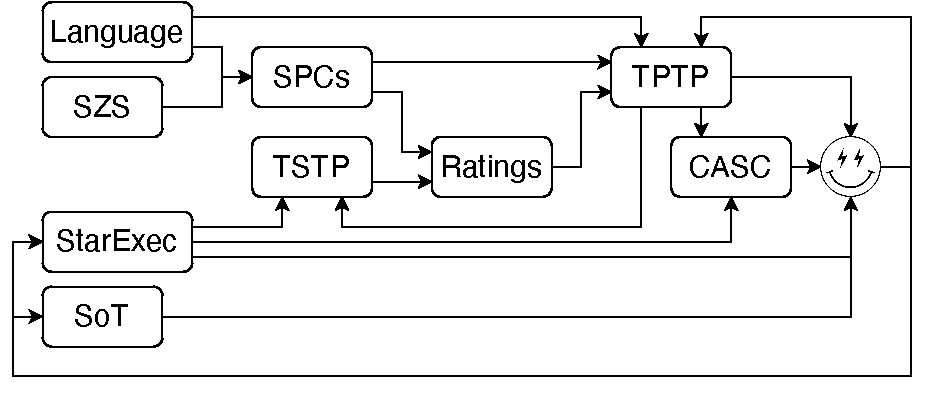
\includegraphics[width=0.75\textwidth]{Dependencies.pdf}
\caption{Dependencies between the Stepping Stones}
\label{Dependencies}
\end{figure}

Various parts of the TPTP World have been deployed in a range of applications, in both academia 
and industry.
Since the first release of the TPTP problem library in 1993, many researchers have used the 
TPTP World as an appropriate and convenient basis for ATP system research and development. 
Over the years the TPTP World has provided a platform upon which ATP users have presented their 
needs to ATP system developers, who have then adapted their ATP systems to the users’ needs.
The web page {\smalltt{\url{https://www.tptp.org}}} provides access to all components.

\paragraph{This paper is organized as follows:}

%--------------------------------------------------------------------------------------------------
\section{The TPTP Languages}
\label{Languages}

The TPTP language \cite{Sut23-IGPL} is one of the keys to the success of the TPTP World.
The language is used for writing both problems and solutions,
which enables convenient communication between systems. 
% It also enables tool exchange, tool integration, and comparable experimental results.
Originally the TPTP World supported only first-order clause normal form (CNF)
\cite{SS98-JAR}.
Over the years full first-order form (FOF)
\cite{Sut09}, 
typed first-order form (TFF)
\cite{SS+12,BP13-TFF1}, 
typed extended first-order form (TXF)
\cite{SK18}, 
typed higher-order form (THF)
\cite{SB10,KSR16}, 
and non-classical forms (NTF) \cite{SF+22} have been added.
A general principle of the TPTP language is ``we provide the syntax, you provide the semantics''.
As such, there is no a priori commitment to any semantics for the languages, although in almost 
all cases the intended logic and semantics are well known.

The formulae of problems solutions are built from {\em annotated formulae}, 
which have the form~\ldots \\
\hspace*{0.5cm}{\em language}{\tt (}{\em name}{\tt ,}
{\em role}{\tt ,}
{\em formula}{\tt ,}
{\em source}{\tt ,}
{\em useful\_info}{\tt )}\\
The {\em language}s supported are {\smalltt{cnf}} (clause normal form), {\smalltt{fof}}
(first-order form), {\smalltt{tff}} (typed first-order form), and {\smalltt{thf}}
(typed higher-order form).
The {\em role}, e.g., {\smalltt{axiom}}, {\smalltt{lemma}}, {\smalltt{conjecture}}, defines the 
use of the formula in an ATP system.
In a {\em formula}, terms and atoms follow Prolog conventions -- functions and predicates start 
with a lowercase letter or are {\tt '}single quoted{\tt '}, and variables start with an uppercase 
letter.
The language also supports interpreted symbols, which either start with a {\tt \$}, e.g., the 
truth constants {\smalltt{\$true}} and {\smalltt{\$false}}, or are composed of 
non-alphabetic characters, e.g., integer/rational/real numbers such as 27, 43/92, -99.66.
The logical connectives in the TPTP language are
{\tt !}, {\tt ?}, {\tt {\raisebox{0.4ex}{\texttildelow}}}, {\tt |}, {\tt \&}, {\tt =>}, {\tt <=},
{\tt <=>}, and {\tt <{\raisebox{0.4ex}{\texttildelow}}>},
for the mathematical connectives
$\forall$, $\exists$, $\neg$, $\vee$, $\wedge$, $\Rightarrow$, $\Leftarrow$, $\Leftrightarrow$, 
and $\oplus$ respectively.
Equality and inequality are expressed as the infix operators {\tt =} and {\tt !=}.
The {\em source} and {\em useful\_info} are optional.
Figure~\ref{ExampleFormula} shows an example with typed higher-order formulae.

\begin{figure}[htb]
{\footnotesize
{\setlength{\baselineskip}{3mm}
\begin{verbatim}
%------------------------------------------------------------------------------
thf(beverage_decl,type,   beverage: $tType ).
thf(syrup_decl,type,      syrup: $tType ).
thf(coffee_type,type,     coffee: beverage ).
thf(mix_type,type,        mix: beverage > syrup > beverage ).
thf(heat_type,type,       heat: beverage > beverage ).
thf(heated_mix_type,type, heated_mix: beverage > syrup > beverage ).
thf(hot_type,type,        hot: beverage > $o ).

thf(heated_mix,axiom,
    ( heated_mix
    = ( ^ [B: beverage,S: syrup] : ( heat @ ( mix @ B @ S ) ) ) ) ).

thf(hot_mixture,axiom,
    ! [B: beverage,S: syrup] : ( hot @ ( heated_mix @ B @ S ) ) ).

thf(heated_coffee_mix,axiom,
    ! [S: syrup] : ( ( heated_mix @ coffee @ S ) = coffee ) ).

thf(hot_coffee,conjecture,
    ? [Mixture: syrup > beverage] :
      ~ ? [S: syrup] :
          ( ( ( Mixture @ S ) = coffee )
          & ( hot @ ( Mixture @ S ) ) ) ).
%------------------------------------------------------------------------------
\end{verbatim}
}}
\caption{THF annotated formulae}
\label{ExampleFormula}
\end{figure}

%--------------------------------------------------------------------------------------------------
\section{The TPTP Problem Library}
\label{TPTP}

The development of the TPTP World started with the TPTP problem library in mid-1992, as a 
collaboration between Geoff Sutcliffe at the University of Western Australia (James Cook 
University from 1993), and Christian Suttner at the Technische Universit{\"a}t M{\"u}nchen.
The TPTP problem library is managed in the manner of a software product, in the sense that fixed 
releases are made.
Each release is identified by a release number in the form v$Version$.$Edition$.$Patch$:
the $Version$ enumerates major new releases of the TPTP in which important new features have 
been added,
the $Edition$ is incremented each time new problems are added to the current version, and
The $Patch$ level is incremented each time errors, found in the current edition, are corrected. 
The first public release, TPTP v1.0.0, was made on 12th November 1993.

The problems in the TPTP are classified into {\em domains} that reflect the natural hierarchy of 
scientific domains.
Seven main fields are defined: logic, mathematics, computer science, science \& engineering, 
social sciences, arts \& humanities, and other. 
Each field is subdivided into domains, each identified by a three-letter mnemonic, e.g., the
social science field has three domains: Social Choice Theory (SCT), Management (NGT), and
Geography (GEG).

Table~\ref{tab:Releases} lists the versions of the TPTP up to v9.0.0, with the new feature added, 
the number of problem domains, and the number of problems.\footnote{%
The data for v9.0.0 is an estimate, because this paper was written before the release was
finalised.}
The number of domains indicates the semantic diversity of the TPTP problems, while the number
of problems indicates the size of the TPTP problem library.
The attentive reader might note that many releases have been made in July/August.
This is because the CADE ATP System Competition (CASC - see Section~\ref{CASC}), has an 
influence on the release cycle of the TPTP. 

\begin{table}[htb]
\begin{center}
\setlength{\tabcolsep}{4pt}
\begin{tabular}{ll|l|rr}
Release & Date     & Changes                                              & Domains & Problems \\
\hline
v1.0.0  & 12/11/93 & First public release, only CNF \cite{SS98-JAR}       &      23 &     2295 \\
v2.0.0  & 05/06/97 & FOF \cite{Sut09} and ratings (Section~\ref{Ratings}) &      28 &     3277 \\
v3.0.0  & 11/11/04 & New TPTP language \cite{SS+06}                       &      32 &     7267 \\
v4.0.0  & 04/07/09 & TH0 (monomorphic typed higher-order) \cite{SB10}     &      41 &    16512 \\
v5.0.0  & 16/09/10 & TF0 (monomorphic typed first-order) \cite{SS+12}     &      45 &    18480 \\
v6.0.0  & 21/09/13 & TF1 (polymophic typed first-order) \cite{BP13-TFF1}  &      48 &    20306 \\
v7.0.0  & 24/07/17 & TH1 (polymophic typed higher-order) \cite{KSR16}     &      53 &    21851 \\
v8.0.0  & 19/04/22 & TXF (typed extended first-order) \cite{SK18}         &      54 &    24785 \\
v9.0.0  & ??/07/24 & NTF (non-classical typed first-order) \cite{SF+22}   &      55 &    25598 \\
\end{tabular}
\end{center}
\caption{Overview of TPTP releases}
\label{tab:Releases}
\end{table}

TPTP problem files present the logical formulae in a format that is both human and machine 
readable, and additionally provide useful information for users.
The file names are built from the domain acronym, a 3 digit problem number, a separator that
indicates the syntax ({\tt -} for CNF, {\tt +} for FOF, {\tt \_} for TFF, {\tt \verb|^|} for THF),
optional digits for the problem size, and a problem version number.
Each file has three sections: a header, optional includes, and the formulae.

The header section contains information for users, formatted as comments in four parts:
the first part identifies and describes the problem;
the second part provides information about occurrences of the problem
in the literature and elsewhere;
the third part provides semantic and syntactic characteristics of the problem;
the last part contains comments and bugfix information.
The include section is optional, and if used contains {\tt include} directives for axiom files,
which in turn have the same three-part format as problem files.
Their inclusion avoids the need for duplication of the formulae in commonly used axiomatizations.
The formula section contains annotated formulae, as described in Section~\ref{Languages}.
Figure~\ref{ExampleHeader} shows an example header and {\tt include} section.
The header fields are self-explanatory, but of particular interest are the {\tt Status} field 
that is explained in Section~\ref{SZS}, the {\tt Rating} field that is explained in 
Section~\ref{Ratings}, and the {\tt SPC} field that is explained in Section~\ref{SPCs}.

\begin{figure}[htb]
{\footnotesize
{\setlength{\baselineskip}{3mm}
\begin{verbatim}
%------------------------------------------------------------------------------
% File     : DAT016_1 : TPTP v8.2.0. Bugfixed v5.1.0.
% Domain   : Data Structures
% Problem  : Some element is 53
% Version  : [PW06] axioms.
% English  : Show that some element of the array has the value 53.

% Refs     : [PW06]  Prevosto & Waldmann (2006), SPASS+T
%          : [Wal10] Waldmann (2010), Email to Geoff Sutcliffe
% Source   : [Wal10]
% Names    : (40) [PW06]

% Status   : Theorem
% Rating   : 0.25 v8.2.0, 0.12 v7.5.0, 0.30 v7.4.0, 0.12 v7.3.0, etc.
% Syntax   : Number of formulae    :    6 (   1 unt;   3 typ;   0 def)
%            Number of atoms       :   12 (   5 equ)
%            Maximal formula atoms :    4 (   2 avg)
%            Number of connectives :    4 (   0   ~;   1   |;   1   &)
%                                         (   0 <=>;   2  =>;   0  <=;   0 <~>)
%            Maximal formula depth :    6 (   5 avg)
%            Maximal term depth    :    3 (   1 avg)
%            Number of FOOLs       :    5 (   5 fml;   0 var)
%            Number arithmetic     :   16 (   2 atm;   2 fun;   5 num;   7 var)
%            Number of types       :    2 (   1 usr;   1 ari)
%            Number of type conns  :    5 (   2   >;   3   *;   0   +;   0  <<)
%            Number of predicates  :    3 (   1 usr;   0 prp; 2-2 aty)
%            Number of functors    :    9 (   2 usr;   5 con; 0-3 aty)
%            Number of variables   :   10 (   9   !;   1   ?;  10   :)
% SPC      : TF0_THM_EQU_ARI

% Comments : The array contains integers.
% Bugfixes : v5.1.0 - Fixed conjecture
%------------------------------------------------------------------------------
%----Includes axioms for arrays
include('Axioms/DAT001_0.ax').
%------------------------------------------------------------------------------
\end{verbatim}
}}
\caption{Header of problem {\tt DAT016\_1}.}
\label{ExampleHeader}
\end{figure}


This section has naturally focused on the successful parts of the TPTP history.
There have also been some failed developments and suboptimal (in retrospect) decisions \frownie{}.
For example, in 2015 there was an attempt to develop a description logic form for the TPTP 
language. 
While some initial progress was made, it ground to a halt without support from the description 
logic community.
A suboptimal design decision, rooted in the early days of the TPTP, is the naming scheme used for 
problem files. 
The naming scheme uses three digits to number the problems in each domain, thus setting a limit 
of 1000 problems, which failed to anticipate the numbers of problems that would be contributed 
to some of the problem domains.
This has been overcome by creating multiple domain directories where necessary, but if it were 
to be done again, six or eight digit problem numbers shared across all domains would be an 
improvement.

%--------------------------------------------------------------------------------------------------
\section{The TSTP Solution Library}
\label{TSTP}

The complement of the problem library is the TSTP solution library \cite{Sut07-CSR,Sut10}.
% Started as the results collection for the TPTP circa 1997, became the TSTP circa 2002.
The TSTP is built by running all the ATP systems that are available in the TPTP World on
all the problems in the TPTP problem library.
% The ATP systems come from a range of sources:
% some were developed many years ago and are no longer distributed;
% some are the most recent available, taken either from the systems’ web sites or from the most 
% recent edition of CASC.
At the time of writing this paper, the TSTP contained the results of running 87 ATP systems and 
system variants on all the problems in the TPTP that they could attempt
(therefore, e.g., systems that do model finding for FOF are not run on THF problems).
This produced 1091026 runs, of which 432718 (39.6\%) solved the problem.

Since 2014 the ATP systems have been run on StarExec \cite{SST14}, initially on the StarExec
Iowa cluster, and since 2018 on the StarExec Miami cluster (see Section~\ref{StarExec}.
StarExec has provided stable platforms that produce reliably consistent and comparable data in
the TSTP.
Analysis shows that increasing resource limits does not significantly affect which problems 
are solved by an ATP system. 
Figure~\ref{PPPPlot} illustrates this point; it plots the CPU times taken by several contemporary 
ATP systems to solve the TPTP problems for the {\tt FOF\_THM\_RFO\_*} SPCs, in increasing order 
of time taken. 
The data was taken from the TSTP, i.e., using the StarExec Miami computers.
The relevant feature of these plots is that each system has a point at which the time taken to 
find solutions starts to increase dramatically. 
This point is called the system's Peter Principle \cite{PH69} Point (PPP), as it is the point at 
which the system has reached its level of incompetence. 
Evidently a linear increase in the computational resources beyond the PPP would not lead to the 
solution of significantly more problems. 
The PPP thus defines a realistic computational resource limit for the system. 
% From an ATP perspective, the PPP is the point at which the ATP system gets lost in its quickly 
% growing search space. 
% Even though there may be enough memory to represent the search space at the PPP, the system is 
% largely unable to find a solution within the space. 
% The point thus also defines a realistic memory resource limit. 
Therefore, provided that enough CPU time and memory are allowed for an ATP system to reach its 
PPP, a usefully accurate measure of what problems it can solve is achieved.
The performance data in the TSTP is produced with adequate resource limits.

\begin{figure}[t!]
\centering
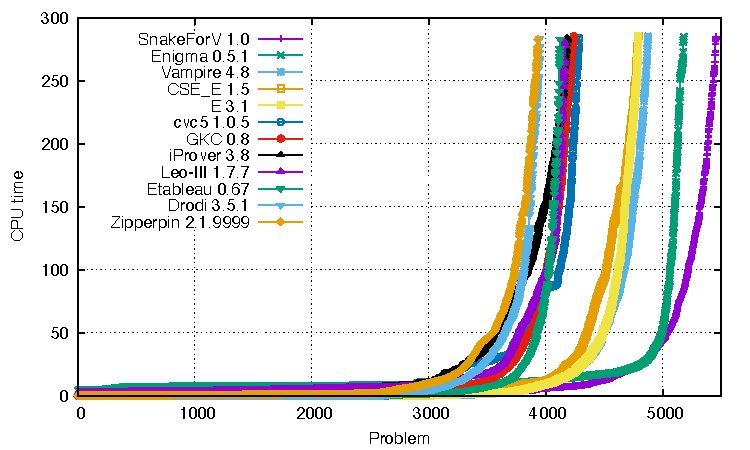
\includegraphics[width=0.6\textwidth]{FOF_THM_RFO_PPP.pdf}
\vspace*{-1em}
\caption{CPU times for {\tt FOF\_THM\_RFO\_*}}
\label{PPPPlot}
\end{figure}

One use of the TSTP is for ATP system developers to examine solutions to problems and thus 
understand how they can be solved, leading to improvements to their own systems. 
Another use is for computing the TPTP problem ratings (see Section~\ref{Ratings}).

%--------------------------------------------------------------------------------------------------
\section{The SZS Ontologies}
\label{SZS}

The TPTP infrastructure uses the three SZS ontologies to help facilitate 
automatic processing of TPTP problems and ATP systems' output 
\cite{Sut08-KEAPPA} (named ``SZS'' after the authors of the first 
presentation of the ontologies \cite{SZS03}).
The ontologies provide values to specify the logical status of problems, and 
to describe logical data.
Figure~\ref{SZS} shows some of the salient nodes of the ontologies.
The Success ontology provides values for the logical status of a conjecture 
with respect to a set of axioms, e.g., a TPTP problem whose conjecture is a
logical consequence of the axioms is tagged as a {\tt Theorem} (as in 
Figure~\ref{ExampleHeader}), and a model finder that establishes that a set 
of axioms is consistent should report {\tt Satisfiable}.
The Success ontology can also be used to specify the semantic relationship 
between the parents and inferred formula of an inference, as done in TPTP 
format derivations \cite{SS+06} (see Section~\ref{TPTP} for an example).
The NoSuccess ontology catalogs reasons why an ATP system/tool has failed,
e.g., an ATP system might report {\tt Timeout}.
The Dataform ontology provides values for describing the form of logical data,
as might be output from an ATP system/tool, e.g., a model finder might output 
a {\tt FiniteModel}.
The SZS standard also recommends the precise way in which the ontology values 
should be presented in ATP system output, in order to facilitate easy 
processing.

\begin{figure}[bht]
\begin{center}
\mbox{} 
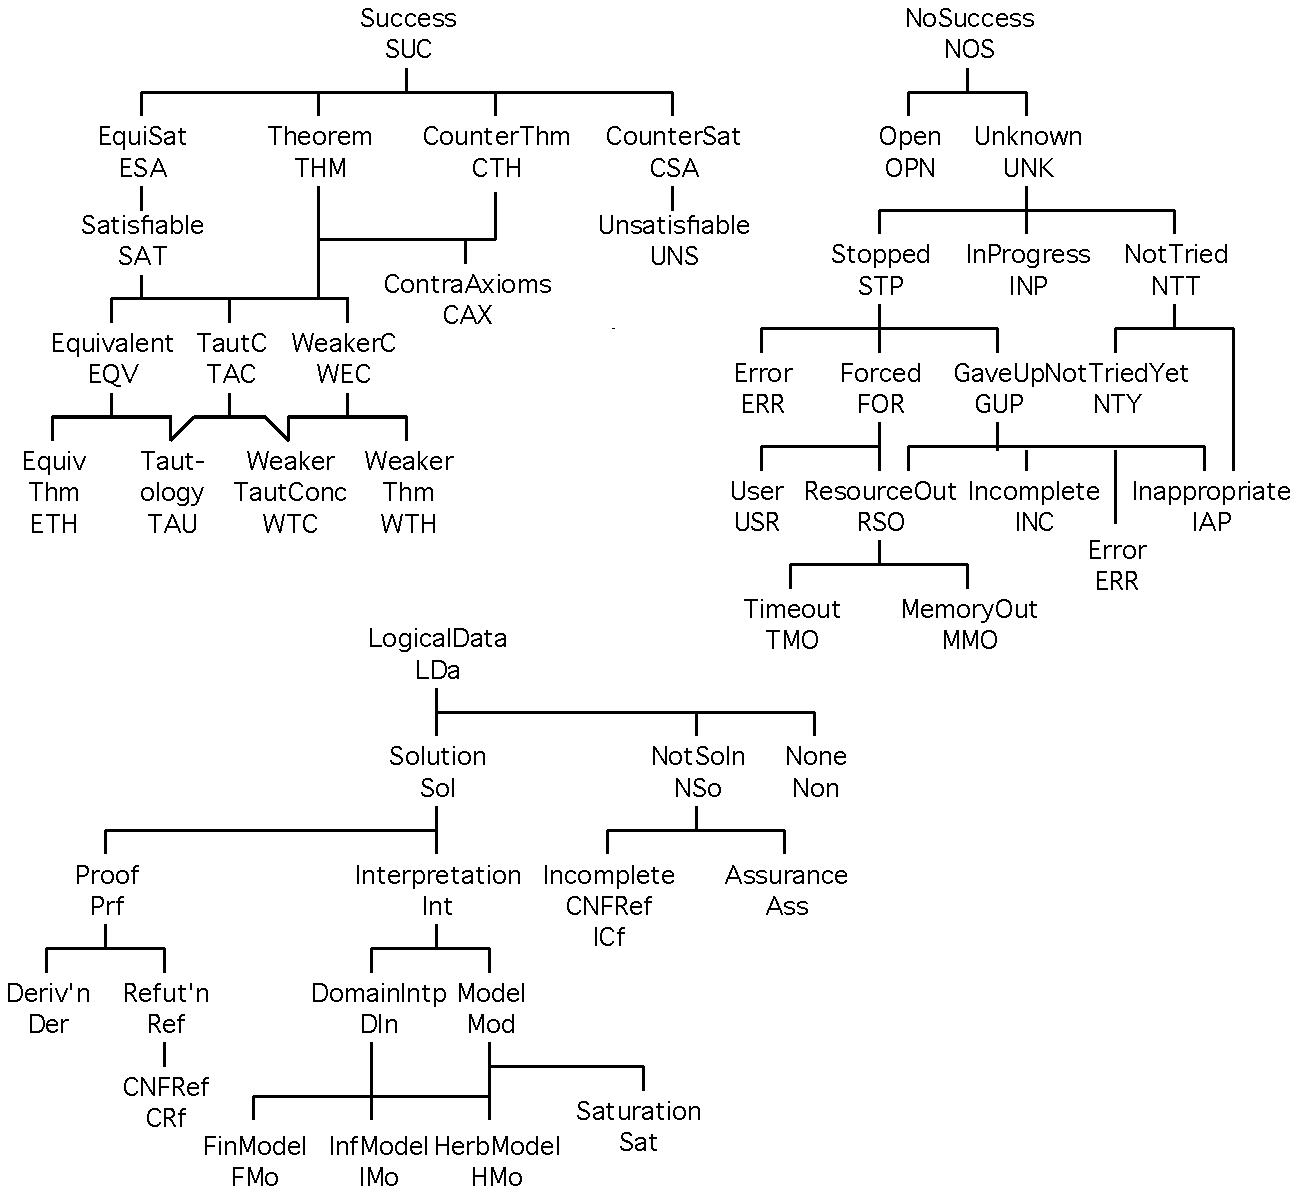
\includegraphics[width=0.75\textwidth]{SZSOntologies.pdf}
\caption{The SZS ontologies}
\label{SZS}
\end{center}
\end{figure} 

%--------------------------------------------------------------------------------------------------
\section{Specialist Problem Classes}
\label{SPCs}

The problems in the TPTP library are divided into Specialist Problem Classes (SPCs) -- classes of 
problems that are homogeneous wrt recognizable logical, language, and syntactic characteristics.
% SPCs added in v4.1.0 15/06/10
Evaluation of ATP systems within SPCs makes it possible to say which systems work well for what 
types of problems. 
The appropriate level of subdivision for SPCs is that at which less subdivision would merge 
SPCs for which ATP systems have distinguishable behaviour, and at which further subdivision
would unnecessarily split an SPC for which ATP systems have reasonably homogeneous behaviour.
Empirically, homogeneity is ensured by examining the patterns of system performance across the 
problems in each SPC. 
For example, the separation of ``essentially propositional'' problems was motivated by observing 
that SPASS \cite{WA+99} performed differently on the ALC problems in the SYN domain of the TPTP.
A data-driven test of homogeneity is also possible \cite{FS02}.

The characteristics currently used to define the SPCs in the TPTP are~\ldots
\begin{packed_itemize}
\item TPTP language: \\
      {\tt CNF} -- Clause Normal Form
      {\tt FOF} -- First-Order Form \\
      {\tt TF0} -- Typed Monomorphic First-order form \\
      {\tt TF1} -- Typed Polymorphic First-order form \\
      {\tt TX0} -- Typed Monomorphic eXtended First-order form \\
      {\tt TX1} -- Typed Polymorphic eXtended First-order form \\
      {\tt TH0} -- Typed Monomorphic Higher-order form \\
      {\tt TH1} -- Typed Polymorphic Higher-order form
\item SZS status: \\
      \begin{tabular}{@{}p{5cm}l}
      {\tt THM} -- Theorem &
      {\tt CSA} -- CounterSAtisfiable \\
      \multicolumn{2}{@{}l}{{\tt CAX} -- Contradictory AXioms (merged with {\tt THM} in this work)} \\
      {\tt UNS} -- UNSatisfiable &
      {\tt SAT} -- SATisfiable \\
      {\tt UNK} -- UNKown &
      {\tt OPN} -- OPeN \\
      \end{tabular}
\item Order (for {\tt CNF} and {\tt FOF}): \\
      {\tt PRP} -- PRoPositional \\
      {\tt EPR} -- Effectively PRopositional (known to be reducible to {\tt PRP}) \\
      {\tt RFO} -- Real First-Order (not known to be reducible to {\tt PRP})
\item Equality: \\
      \begin{tabular}{@{}p{5cm}l}
      {\tt NEQ} -- No EQuality &
      {\tt EQU} -- EQUality (some or pure) \\
      {\tt SEQ} -- Some (not pure) EQUality &
      {\tt PEQ} -- Pure EQUality \\
      {\tt UEQ} -- Unit EQUality {\tt CNF} &
      {\tt NUE} -- Non-Unit Equality {\tt CNF} \\
      \end{tabular}
\item Hornness (for {\tt CNF}): \\
      \begin{tabular}{@{}p{5cm}l}
      {\tt HRN} -- HoRN &
      {\tt NHN} -- Non-HorN
      \end{tabular}
\item Arithmetic (for {\tt T*} languages): \\
      \begin{tabular}{@{}p{5cm}l}
      {\tt NAR} -- No ARithmetic &
      {\tt ARI} -- ARIthmetic.
      \end{tabular}
\end{packed_itemize}

Using these characteristics 223 SPCs are defined in TPTP v8.2.0. 
For example, the SPC
% Some examples are:
% {\tt CNF\_SAT\_EPR\_PEQ\_UEQ} -- clause normal form satisfiable clauses that are effectively
% propositional, have purely equality literals in unit equality clauses;
% {\tt FOF\_THM\_RFO\_SEQ} -- first-order theorems that are ``really first-order'' (not known
% to be effectively propositional), and contain some (not only) equality;
{\tt TF0\_THM\_NEQ\_ARI} contains typed monomorphic first-order theorems that have no equality but 
include arithmetic.
The header section of each problem in the TPTP problem library (see Section~\ref{TPT}) includes 
its SPC.

The SPCs are used when computing the TPTP problems difficulty ratings, as explained in
Section~\ref{Ratings}.

%--------------------------------------------------------------------------------------------------
\section{Problem Difficulty Ratings}
\label{Ratings}

Each TPTP problem has a difficulty rating that provides a well-defined measure of how difficult 
the problem is for current ATP systems \cite{SS01}.
The ratings are based on performance data in the TSTP (see Section~\ref{TSTP}), and are updated
in each TPTP edition.
Rating is done separately for each SPC.
First, a partial order between systems is determined according to whether or not a system 
solves a strict superset of the problems solved by another system. 
If a strict superset is solved, the first system is said to {\em subsume} the second. 
% The union of the problems solved by the non-subsumed systems defines the state-of-the-art -- all 
% the problems that are solved by any system. 
Then the fraction of non-subsumed systems that fail on a problem is the difficulty rating 
for the problem. 
Problems that are solved by all of the non-subsumed systems get a rating of 0.00 (``easy'');
problems that are solved by some of the non-subsumed systems get a rating between 
0.00 and 1.00 (``difficult''); 
problems that are solved by none of the non-subsumed systems get a rating of 1.00 (``unsolved'').

%--------------------------------------------------------------------------------------------------
\section{StarExec and SystemOnTPTP}
\label{StarExec}

The StarExec Miami computers have an
octa-core Intel Xeon E5-2667 v4 CPU running at 2.10 GHz,
128 GiB memory,
and the CentOS Linux release 7.4.1708 operating system.
% Linux kernel 3.10.0-1160.62.1.el7.x86\_64.
One ATP system is run on one CPU at a time, with a 300s CPU time limit and a 128GiB memory
limit.

%--------------------------------------------------------------------------------------------------
\section{The CADE ATP System Competition}
\label{CASC}

The CADE ATP System Competition (CASC) \cite{Sut16} is the annual evaluation of fully automatic,
classical logic, ATP systems - the world championship for such systems.
One purpose of CASC is to provide a public evaluation of the relative capabilities of ATP systems.
Additionally, CASC aims to
stimulate ATP research,
motivate development and implementation of robust ATP systems that can be easily and usefully
deployed in applications,
provide an inspiring environment for personal interaction between ATP researchers,
and
expose ATP systems within and beyond the ATP community.
CASC evaluates the performance of the ATP systems in terms of
the number of problems solved,
the number of acceptable solutions (proofs or models) output, and
the average time taken for problems solved,
in the context of
a bounded number of eligible problems and
specified time limits.

CASC is held at each CADE (the International Conference on Automated Deduction) and IJCAR
(the International Joint Conference on Automated Reasoning) conference -- the major forums
for the presentation of new research in all aspects of automated deduction.
Over the years CASC has been a catalyst for impressive improvements in ATP, stimulating both 
theoretical and implementation advances \cite{Nie02-Paper}.
It has provided a forum at which empirically successful implementation efforts are acknowledged 
and applauded, and at the same time provides a focused meeting at which novice and experienced 
developers exchange ideas and techniques. 
The CASC web site provides access to all the details:
\href{http://www.tptp.org/CASC/}{{\tt www.tptp.org/CASC}}.

The first CASC was held at CADE-13 in 1996, at DIMACS in Rutgers University, USA, in collaboration
with Christian Suttner.
Of particular interest for this IJCAR is that CASC was conceived of in 1994 after CADE-12 in
Nancy, when we were sitting on a bench under a tree in Parc de la Pépinière, burning time before
our train departures.

CASC is run in divisions according to problem and system characteristics. 
Over the years the following divisions have existed (those marked with an
* are the divisions for CASC-25):
\begin{packed_itemize}
\item THF$^*$: 
      {\bf T}yped {\bf H}igher-order {\bf F}orm theorems (axioms with a 
      provable conjecture).
\item THN$^*$: 
      {\bf T}yped {\bf H}igher-order form {\bf N}on-theorems (axioms 
      with a countersatisfiable (i.e., unprovable) conjecture, and 
      satisfiable axiom sets).
\item TFA$^*$: 
      {\bf T}yped {\bf F}irst-order with {\bf A}rithmetic theorems (axioms 
      with a provable conjecture).
\item TFN$^*$: 
      {\bf T}yped {\bf F}irst-order with arithmetic {\bf N}on-theorems 
      (axioms with a countersatisfiable conjecture, and satisfiable axiom sets).
\item FOF$^*$: 
      {\bf F}irst-{\bf O}rder {\bf F}orm theorems (axioms with a provable 
      conjecture). 
\item FNT$^*$: 
      {\bf F}irst-order form {\bf N}on-{\bf T}heorems (axioms with a 
      countersatisfiable conjecture, and satisfiable axiom sets).
\item CNF:
      {\bf C}lause {\bf N}ormal {\bf F}orm theorems (unsatisfiable clause 
      sets) that are not effectively propositional\footnote{%
      {\em Effectively propositional} means that the problem is known to be 
      reducible to a propositional problem, e.g., a CNF problem that has no 
      functions with arity greater than zero.}, and not unit equality 
      problems (see the UEQ division below).
\item SAT:
      {\bf C}lause {\bf N}ormal {\bf F}orm non-theorems (satisfiable clause 
      sets) that are not effectively propositional, and not unit equality 
      problems (see the UEQ division below).
\item EPR$^*$: 
      {\bf E}ffectively {\bf PR}opositional theorems and non-theorems
      (unsatisfiable and satisfiable clause sets).
\item UEQ:
      {\bf U}nit {\bf EQ}uality theorems (unsatisfiable clause
      sets) that are not effectively propositional.
\item SEM:
      FOF theorems based on a specified axiomatization of a specified
      {\bf SEM}antic domain.
\item LTB$^*$: 
      First-order form theorems (axioms with a provable 
      conjecture) from {\bf L}arge {\bf T}heories, presented in {\bf B}atches
      with a shared time limit.
\end{packed_itemize}

% Some of the divisions are further divided into problem categories, which
% makes it possible to analyze, at a more fine grained level, which systems
% work well for what types of problems.
% The problem categories have no effect on the competition rankings, which
% are made at only the division level.
The different logics and syntactic characteristics of the problems in the
various divisions provide different challenges for ATP systems. 
The tasks of proving theorems and showing unsatisfiability (which can
be treated similarly) are quite distinct from establishing non-provability 
and satisfiablility (which can also be treated similarly).

Problems for CASC are taken from the TPTP Problem Library. 
The TPTP version used for CASC is released after the competition,
so that new problems have not been seen by the entrants. 
In some divisions the systems are ranked according to the number of problems 
solved with an acceptable proof/model output, and some divisions the systems
are ranked according to the number of problems solved but not necessarily 
accompanied by a proof or model
(thus giving only an assurance of the existence of a proof/model). 
Ties are broken according to the average time over problems solved.
Division winners are announced and prizes are awarded.
In addition to the ranking criteria, three other measures are made and
presented in the results:
The {\em state-of-the-art (SoTA) contribution} quantifies the unique
abilities of each system.
For each problem solved by a system, its SoTA contribution for the problem 
is the inverse of the number of systems that solved the problem, and
% so that if a system is the
% only one to solve a problem then its SoTA contribution for the problem 
% is 1.00, and if all the systems solve a problem their SoTA contributions for 
% the problem are the inverse of the number of systems.
it's overall SoTA contribution is the average SoTA contribution over 
the problems it solved.
The {\em efficiency measure} is a combined measure that balances the time
taken for each problem solved against the number of problems solved.
It is the average of the inverses of the times for problems solved,
This can be interpreted intuitively as the average of the solution rates
for problems solved, multiplied by the fraction of problems solved.
The {\em core usage} is the average of the ratios of CPU time to
wall clock time used, over the problems solved.
This measures the extent to which the systems take advantage of multiple cores.

CASC typically has 20 to 30 ATP systems entered.
For each CASC the division winners of the previous CASC are automatically
entered to provide benchmarks against which progress can be judged.
Additionally, a fixed version (initially v3.2, later v3.3) of the well known 
Otter ATP system was entered in every CASC from 2002 to 2011, as a fixed 
point against which progress could be judged.
By 2011 Otter was no longer competitive, and was replaced by Prover9 2009-11A
in 2012.
Over all 20 CASCs so far 99 distinct ATP systems have been entered.
Almost all the ATP systems have come from academia, partially due to the
CASC requirement that all source code must be published on the CASC web site.
The most popular divisions have been the FOF, FNT, CNF, SAT, EPR, and 
UEQ divisions.
Some systems have emerged as dominant in some of the divisions:
Satallax in the THF division, Vampire in the FOF and CNF divisions, Paradox
in the FNT and SAT divisions (with iProver now coming on strong), iProver
in the EPR division, and Waldmeister in the UEQ division.
The strengths of these systems stem from four main areas:
solid theoretical foundations, significant implementation efforts (in terms
of coding and data structures), extensive testing and tuning, and an
understanding of how to optimize for CASC.
For example, Vampire is founded on the theoretical principles of 
superposition, has a highly efficient implementation in C++ using code
trees and advanced structures for representing logical data, is repeatedly
tested and tuned on the TPTP problem library, and has special modes for
the various divisions of CASC.
Technical information about these systems, and the techniques they employ,
can be found on the individual CASC web pages.

The design and organization of CASC has evolved over the years to a 
sophisticated state.
Decisions made for CASC (alongside the TPTP) have had an influence on the 
directions of development in ATP.
It is interesting to look back on some of the key decisions that have helped 
bring the competition to its current state.
\begin{packed_itemize}
\item CASC-13, 1996: The first CASC stimulated research towards robust,
    fully automatic systems that take only logical formulae as input.
    It increased the visibility of systems and developers, and rewarded 
    implementation efforts.
\item CASC-14, 1997: Introduced the SAT division, stimulating the 
    development of model finding systems for CNF.
%    Gandalf demonstrated the great benefits of strategy scheduling,
%    which has evolved into a standard approach in ATP.
\item CASC-15, 1998: Introduced the FOF division, starting the slow demise 
    of CNF to becoming just the ``assembly language'' of ATP. 
\item CASC-16, 1999: Changes to the problem selection process motivated the 
    development of techniques for automatic tuning of ATP systems' search
    parameters.
% \item CASC-17, 2000: Systems had to be delivered as a ``installation 
%     package'', hoping to make ATP systems easier for users to install 
%     and use.
\item CASC-JC, 2001: Introduced ranking based on proof output, starting the
    the trend towards ATP systems that efficiently output proofs and models.
    Introduced the EPR division, stimulating the development of specialized
    techniques for this important subclass of problems.
% \item CASC-18, 2002:
% \item CASC-19, 2003:
% \item CASC-J2, 2004:
\item CASC-20, 2005: Required systems to develop builtin equality reasoning,
    by removing the equality axioms from all TPTP  problems.
\item CASC-J3, 2006: The FOF division was promoted as the most important,
    stimulating development of ATP systems for full first-order logic.
\item CASC-21, 2007: Introduced the FNT division, further stimulating the
    development of model finding systems.
\item CASC-J4, 2008: Introduced the LTB division, stimulating the development
    of techniques for automatically dealing with very large axiom sets.
% \item CASC-22, 2009: 
\item CASC-J5, 2010: Introduced the THF division, stimulating development
    of ATP systems for higher-order logic.
\item CASC-23, 2011: Introduced the TFA division, stimulating development
    of ATP systems for full first-order logic with arithmetic.
\item CASC-J6, 2012: Otter replaced by Prover9 as the ``fixed-point'' in the
    FOF division, demonstrating the progress in ATP.
\item CASC-24, 2013: Removed the CNF division, confirming the demise of CNF.
\item CASC-J7, 2014: Required use of the SZS ontology, so the ATP systems 
    unambiguously report what they have established about the problem.
\item CASC-25, 2015: Introduced the THN and TFN divisions, stimulating
    development of model finding for the THF and TFA logics.
\end{packed_itemize}

Over the years the TPTP and CASC have increasingly been used as a conduit 
for ATP users to provide samples of their problems to ATP system developers.
Users' problems that are contributed to the TPTP are eligible for use
in CASC.
The problems are then exposed to ATP system developers, who improve their 
systems' performances on the problems, in order to perform well in CASC.
This completes a cycle that provides the users with more effective tools
for solving their problems.
%--------------------------------------------------------------------------------------------------
\section{TPTP World Users}
\label{Users}

%--------------------------------------------------------------------------------------------------
\section{Conclusion}
\label{Conclusion}

This paper 

Currently this work is being extended to 

%--------------------------------------------------------------------------------------------------
\bibliographystyle{plain}
\bibliography{Bibliography.bib}
%--------------------------------------------------------------------------------------------------
\end{document}
%--------------------------------------------------------------------------------------------------
